%!TeX root = ../../Tesi.tex
\nocite{MathWorksParallelComputing}
Il Parallel Computing Toolbox, abbreviato in PCT, permette di risolvere problemi \textit{compute-intesive} e  \textit{data-intensive} sfruttando 
la capacit\`a di calcolo offerta dai pi\`u recenti sistemi \textit{multicore} e \textit{cluster} di elaboratori. \newline
Costrutti di programmazione di alto livello, come gli \textit{array} distribuiti, consentono di sviluppare applicazioni MATLAB scalabili senza ricorrere alla programmazione 
MPI\footnote{La \textit{Message Passing Interface} (MPI) rappresenta lo standard per il modello di comunicazione interprocesso basato sullo scambio 
di messaggi nei sistemi distribuiti\,\cite{NMSUMPIIntro}, stabilendo la sintassi e la semantica di funzioni di libreria impiegate nella scrittura di software parallelo in C, \CC e Fortran.}.\newline
L'applicazione pu\`o essere eseguita su \textit{cluster} o su server in \textit{cloud} senza dover apportare alcuna modifica al codice grazie a MATLAB 
Parallel Server, cos\`i da concentrarsi esclusivamente sullo sviluppo dell'algoritmo migliore per il caso d'uso in esame.

Incominciamo il nostro studio del Parallel Computing Toolbox riportando alcune definizioni, tratte dalla documentazione ufficiale di MATLAB\,\cite{MathWorksWhatIsParallel}, riguardanti il modello di programmazione parallela messo a disposizione dal linguaggio.
\begin{itemize}
\item \textit{Client}: termine impiegato per identificare la sessione di MATLAB con cui l'utente sta interagendo; tipicamente coincide con il 
computer usato dallo sviluppatore durante la prototipazione del programma a esecuzione parallela.\newline
Attraverso le funzioni che compongono il PCT, il \textit{client} suddivide la computazione in \textit{task} atomiche e le assegna ai \textit{worker}.
\item \textit{Parallel Pool}: spesso abbreviato in parpool, \`e definito come un insieme di \textit{worker} comunicanti che possono eseguire codice interattivamente.
\item \textit{Worker}: corrisponde a un'istanza di MATLAB priva di interfaccia grafica, in grado di fornire la potenza del 
motore di calcolo del linguaggio.
\end{itemize}

Una prima distinzione da rimarcare \`e quella fra l'infrastruttura e i componenti del linguaggio inclusi negli strumenti di calcolo parallelo di MATLAB.\newline 
Il linguaggio comprende costrutti di programmazione parallela e funzioni con supporto automatico al parallelismo, mentre l'infrastruttura riguarda i meccanismi che coaudivano il linguaggio, come il protocollo di trasferimento del codice e dei dati alle unit\`a di lavoro. \newline
Nelle prossime sezioni, esamineremo da vicino alcuni costrutti paralleli proprio del linguaggio, astraendo dall'infrastruttura sottostante, nonostante entrambe le componenti 
siano imprescindibili per il corretto funzionamento del PCT.

\subsection{L'architettura di riferimento}
L'architettura di un cluster di elaboratori impiegata per l'analisi del Parallel Computing Toolbox \`e schematizzata in figura \ref{fig:ArchitetturaRiferimento}.\newline
MATLAB Parallel Server riunisce un insieme di \textit{worker}, in esecuzione sui nodi del \textit{cluster}, che ricevono le 
\textit{task} computazionali assegnate dal \textit{client} attraverso specifiche funzioni del Parallel Computing Toolbox. \newline
I \textit{worker} leggono il codice da eseguire e i dati su cui lavorare da una memoria di massa condivisa popolata dall'\textit{head node} 
(non rappresentato in figura), un nodo del sistema responsabile della schedulazione delle attivit\`a.\newline
Una volta terminata l'elaborazione, i risultati sono raccolti dall'\textit{head node} e posti all'interno dello spazio di lavoro del \textit{client} 
mediante i canali di comunicazione instaurati tra quest'ultimo e i \textit{worker}.

\begin{figure}[htbp]
    \centering
    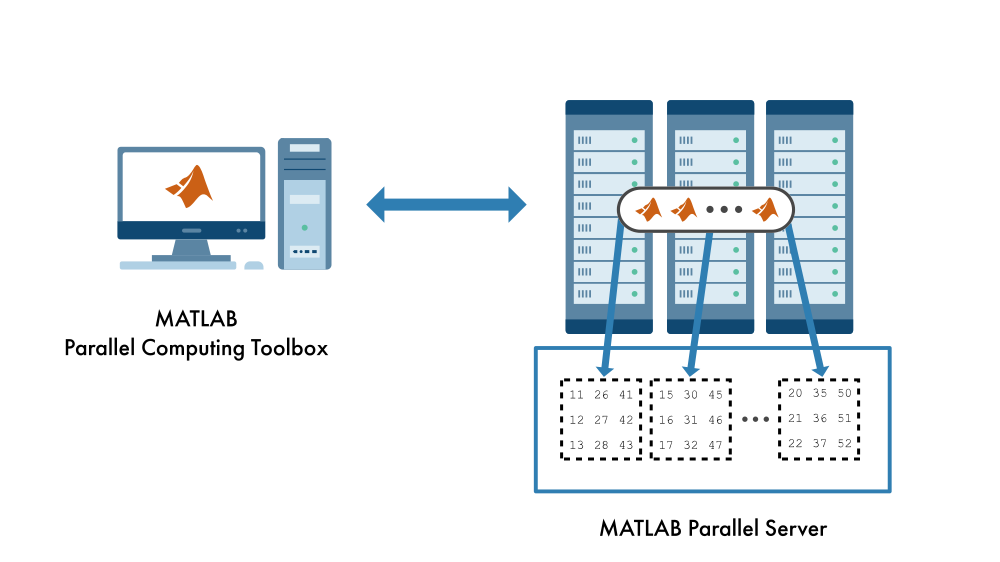
\includegraphics[width=0.8\textwidth]{../Risorse/Capitolo 2/ReferenceArchitecture.png}
    \caption{Architettura di riferimento per gli strumenti di calcolo parallelo di MATLAB. 
    \small{(Da \url{https://it.mathworks.com/products/matlab-parallel-server.html})}}
    \label{fig:ArchitetturaRiferimento}
\end{figure}

Giunti a questo punto, introduciamo i paradigmi di programmazione parallela supportati da MATLAB:
\begin{itemize}
    \item parallelizzazione implicita: alcune funzioni, quando richiamate dal codice sorgente del programma, sfruttano le librerie di \textit{runtime} del linguaggio 
    in modo da essere eseguite su \textit{thread} distinti all'interno della stessa sessione;
    \item parallelizzazione esplicita: il carico di lavoro del programma \`e automaticamente suddiviso in \textit{task} elementari, ciascuna delle quali viene 
    attribuita a un \textit{worker} per l'esecuzione.
\end{itemize}

\nocite{MathWorksParallelQuickStart}
\subsection{Il paradigma di programmazione parallela implicita}
I \textit{toolbox} di MATLAB sono dotati di un crescente numero di funzioni con supporto automatico al parallelismo, al fine di beneficiare di tutti 
i vantaggi dati dall'elaborazione parallela senza modificare il codice eventualmente scritto per la versione seriale di un programma, in accordo con i principi di design elencati 
nella sezione \ref{sec2.1.2}. 

Alcune funzioni, come \lstinline|mldivide| per la risoluzione di sistemi di equazioni lineari, sono eseguite automaticamente su \textit{thread} 
distinti, se richiamate dalla sessione attiva di MATLAB. 

Ragionando sulla nostra architettura di riferimento, il parallelismo implicito viene attivato solo quando la funzione \`e eseguita direttamente dal \textit{client}, 
mentre \`e sconsigliato quando l'esecuzione \`e a carico dei nodi del \textit{cluster}, allo scopo di evitare un parallelismo \enquote{annidato} che degraderebbe le prestazioni 
dell'intero sistema. \newline
In quest'ottica, possiamo notare come i progettisti del linguaggio abbiano ideato i \textit{worker} come unit\`a di elaborazione a singolo \textit{thread}.

Quando il \textit{client} incontra una funzione con supporto automatico al parallelismo nel codice sorgente del programma, avvia un \textit{parallel pool} per la sua esecuzione in parallelo. \newline
Un apposito profilo di configurazione determina le caratteristiche dell'ambiente di elaborazione parallela; nello specifico, il Parallel Computing Toolbox permette di scegliere tra i 
seguenti profili preimpostati:
\begin{itemize}
    \item \textit{Processes}: i \textit{worker} vengono attivati come processi in esecuzione sui \textit{core} fisici del calcolatore che ospita la sessione 
    principale di MATLAB.
    \item \textit{Threads}: i \textit{worker} sono in esecuzione su dei \textit{thread} e non pi\`u su processi veri e propri.
\end{itemize}
I vantaggi portati dall'ambiente 
parallelo \textit{Threads} sono un minor consumo di memoria, un basso costo di comunicazione tra i \textit{worker} e una schedulazione delle attivit\`a particolarmente 
performante, a scapito della disponibilit\`a di un'ampia gamma di funzioni con supporto al parallelismo implicito su \textit{thread}.

Relativamente alla scelta del numero di \textit{worker} nell'ambiente \textit{Processes} \'e consigliato riservare un motore di calcolo per ogni \textit{core} 
fisico disponibile, ignorando la presenza di eventuali \textit{core} virtuali; infatti, questi ultimi condividono alcune risorse di calcolo appartenenti allo 
stesso processore, tra cui la \textit{Floating Point Unit} (FPU), e poich\'e la maggior parte delle elaborazioni in MATLAB richiede l'esecuzione di operazioni 
aritmetiche in virgola mobile, limitare il numero di \textit{worker} per CPU a uno migliora la stabilit\`a del sistema. \newline 
L'unica eccezione \`e rappresentata dalle applicazioni \textit{data-intensive}, per le quali potrebbe essere conveniente innalzare il numero di \textit{worker} per 
\textit{core} a due.

Indipendentemente dall'ambiente di esecuzione selezionato, un singolo parpool a supporto della parallelizzazione implicita pu\`o contenere fino a 512 \textit{worker}, a prescindere dalle specifiche 
del calcolatore utilizzato.
\begin{figure}[htbp]
    \centering
    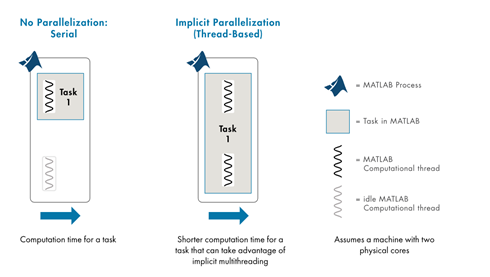
\includegraphics[width=0.8\textwidth]{../Risorse/Capitolo 2/ImplicitParallelization.png}
    \caption{Rappresentazione del modello di parallelizzazione implicita di MATLAB su un sistema \textit{dual-core}
    \small{(Da \url{https://it.mathworks.com/discovery/matlab-multicore.html})}}
    \label{fig:ParallelismoImplicito}
\end{figure}\newline
Se una funzione non include il supporto automatico al parallelimo, possiamo trasferire l'esecuzione del programma su una \textit{workstation}, in modo da beneficiare 
dello \textit{speedup} garantito da un sistema con maggiore capacit\`a di calcolo, oppure possiamo utilizzare il paradigma di programmazione parallela esplicita offerto 
da MATLAB.

\subsection{Il paradigma di programmazione parallela esplicita}

Il modello di programmazione parallela esplicita esposto dal Parallel Computing Toolbox \`e un'applicazione del parallelismo a livello dei dati, che si fonda sull'esistenza di costrutti di programmazione 
parallela di cui i programmatori possono avvalersi durante il processo di sviluppo.\newline
Il meccanismo a bassissimo livello per la scrittura di programmi a elaborazione parallela \`e la comunicazione basata su scambio di messaggi tra \textit{worker} 
appertenenti al medesimo \textit{parallel pool}, ma questo approccio viene spesso criticato essendo considerato l'equivalente del linguaggio 
Assembly per il calcolo parallelo.\newline
Con l'obiettivo di agevolare la scrittura di software parallelo, alcuni costrutti di programmazione di alto livello sono stati introdotti nel linguaggio, aumentando il livello di 
astrazione del codice e consentendo la scrittura di algoritmi paralleli simili alle loro controparti seriali.

Un esempio di costrutto di alto livello per la programmazione parallela \`e incarnato dagli \textit{array}
\footnote{Secondo la terminologia di MATLAB, la parola \textit{array} \`e un termine universale per riferirsi a strutture dati ospitanti vettori riga, vettori colonna o matrici.} 
distribuiti, strutture dati il cui contenuto viene partizionato tra i \textit{worker} di uno stesso \textit{cluster}.\newline
L'impiego degli \textit{array} distribuiti permette di memorizzare strutture dati di dimensioni tali da non poter essere contenute nella memoria centrale di un 
singolo calcolatore, sfruttando la capacit\`a di memorizzazione offerta dalla combinazione di tutti i nodi del \textit{cluster}.

Gli \textit{array} distribuiti possono contenere dati di qualsiasi tipo e supportano la distribuzione degli elementi lungo una dimensione,  
per riga oppure per colonna.\newline
A questo proposito, dobbiamo precisare che esiste la possibilit\`a di definire distribuzioni dei dati alternative e che, molto spesso, il partizionamento degli elementi viene manipolato implicitamente dall'esecuzione di certe operazioni 
come \lstinline|gather| (una funzione utile a riunire un \textit{array} distribuito all'interno dello spazio di lavoro del \textit{client}).

Un ulteriore vantaggio derivante dall'uso degli \textit{array} distribuiti \`e l'assenza di differenze sintattiche per l'accesso agli elementi rispetto agli \textit{array} tradizionali; l'infrastruttura sottostante garantisce in ogni momento una distribuzione dei dati idonea all'esecuzione delle operazioni 
richieste dall'utente.\newline
Questo ampio raggio di manovra consentito al programmatore potrebbe introdurre consistenti \textit{overhead} di comunicazione tra i \textit{worker}, 
ma sappiamo che la programmabilit\`a rappresenta l'obiettivo di design prioritario nel processo di parallelizzazione di MATLAB, surclassando persino le prestazioni.

Centinaia di funzioni native, e altrettante presenti nei \textit{toolbox} sviluppati dalla \textit{community}, sono state progettate per lavorare sinergicamente con \textit{array} distribuiti.\newline
Ad esempio, MATLAB prevede un enorme insieme di funzioni parallele per l'algebra lineare che operano su \textit{array} distribuiti, implementate a partire dalle procedure definite dalla libreria di algebra lineare numerica ScaLAPACK.